\documentclass{article}
\usepackage{styleFiles/nips10submit_e,times}
\usepackage{amssymb}
\usepackage{amsmath}
\usepackage{epsfig}
\usepackage{wrapfig}
\usepackage[numbers]{natbib}
\usepackage{final/algorithm}
\usepackage{final/algorithmic}
\usepackage{url}
\usepackage{subfigure}

\renewcommand{\baselinestretch}{.99}
  
\newcommand{\comment}[1]{}
\newcommand{\mysection}[1]{\vspace{-4mm}\section{#1}\vspace{-4mm}}
\newcommand{\mysubsection}[1]{\vspace{-3mm}\subsection{#1}\vspace{-3mm}}
\newcommand{\myparagraph}[1]{\vspace{-2mm}\paragraph{#1}}
\newcommand{\mycaption}[1]{\vspace{-3mm}\caption{\em \footnotesize #1}\vspace{-3mm}}
\newcommand{\mytopcaption}[1]{\caption{\em \footnotesize #1}}
\newcommand{\theHalgorithm}{\arabic{algorithm}}
\newcommand{\twofigures}[5]{
\renewcommand{\citename}{\citet}
\begin{minipage}[t]{0.49\textwidth}
\centerline{\psfig{figure=#1,height=#3}}
\end{minipage}\hspace{0.01\textwidth}
\begin{minipage}[t]{0.49\textwidth}
\centerline{\psfig{figure=#2,height=#3}}
\end{minipage}
\raisebox{0mm}
{\makebox[0.5\textwidth][c]{(#4)}\makebox[0.5\textwidth][c]{(#5)}}
}
\newcommand{\threefigures}[4]{
\begin{minipage}[t]{0.32\textwidth}
\centerline{\psfig{figure=#1,height=#4}}
\end{minipage}\hspace{0.01\textwidth}
\begin{minipage}[t]{0.32\textwidth}
\centerline{\psfig{figure=#2,height=#4}}f
\end{minipage}\hspace{0.01\textwidth}
\begin{minipage}[t]{0.32\textwidth}
\centerline{\psfig{figure=#3,height=#4}}
\end{minipage}
}
\newcommand{\threefigurescaps}[7]{
\begin{minipage}[t]{0.32\textwidth}
\centerline{\psfig{figure=#1,height=#4}}
\end{minipage}\hspace{0.01\textwidth}
\begin{minipage}[t]{0.32\textwidth}
\centerline{\psfig{figure=#2,height=#4}}
\end{minipage}\hspace{0.01\textwidth}
\begin{minipage}[t]{0.32\textwidth}
\centerline{\psfig{figure=#3,height=#4}}
\end{minipage}
\raisebox{0mm}
{\makebox[0.32\textwidth][c]{(#5)}\makebox[0.32\textwidth][c]{(#6)}
\makebox[0.32\textwidth][c]{(#7)}
}
}
\newcommand{\argmin}{\operatornamewithlimits{argmin}}
\newcommand{\argmax}{\operatornamewithlimits{argmax}}


\title{CS228 Project: Uncertainty- and Novelty-Based Selection Criteria for Self-Paced Learning in SSVM with Latent Variables}
\date{3/16/2011}
\author{
Laney Kuenzel ~~~~~ Danny Goodman\\
Computer Science Department \\
Stanford University \\
\texttt{\{laney,degoodm\}@cs.stanford.edu}
}


\newcommand{\mthb }{\begin{eqnarray*} }
\newcommand{\mthe }{\end {eqnarray*} }
\newcommand{\ul}{\underline}
\newcommand{\bd}{\textbf}
\newcommand{\prtl}[2]{\frac{\partial #1}{\partial #2}}
\newcommand{\drvt}[2]{\frac{d #1}{d #2}}
\newcommand{\floor}[1]{\lfloor #1\rfloor}

\nipsfinalcopy


\begin{document}

\maketitle
\vspace{-8mm}

\mysection{Introduction}
\label{sec:introduction}
Structural Support Vector Machines (SSVMs) are a type of discriminative classification model that performs well on complex datasets where the form of the feature vector $\Phi(\bf x, \bf y)$ depends on the chosen label $\bf y$ \cite{SSVM}.  Introducing a latent variable $\bf h$ into the feature vector $\Phi(\bf x, \bf y, \bf h)$ further increases the power of the model.  For example, $\bf h$ could be used to mark a region of interest in the input $\bf x$, such as a bounding box of an object in an image, or the location of a protein-binding motif in a DNA sequence.  We call such models \emph{latent SSVMs}.

Latent SSVMs achieve strong results on diverse problems, including motif finding in DNA sequences, natural language processing, handwriting recognition, and object detection \cite{SPL,App1,SSVM}.  Improvements in learning latent SSVMs will therefore have benefits for many applications.

The latent SSVM learning problem is the following \cite{SPL}:

\begin{eqnarray}
&&\min_{{\bf w},\xi_i \geq 0} \frac{1}{2}||{\bf w}||^2 + \frac{C}{n} \sum_{i=1}^n \xi_i, \nonumber \\
\mbox{s.t. } && \max_{h_i \in {\cal H}} {\bf w}^\top \left(\Phi({\bf x}_i,{\bf y}_i,{\bf h}_i) - 
		\Phi({\bf x}_i,\hat{\bf y}_i,\hat{\bf h}_i) \right)
	 \geq \Delta({\bf y}_i,\hat{\bf y}_i) - \xi_i, \nonumber \\
\label{eq:latentSSVM}
&&\forall \hat{\bf y}_i \in {\cal Y}, \forall \hat{h}_i \in {\cal H}, i=1,\cdots,n.
\end{eqnarray}

Intuitively, $\bf w\in\mathbb{R}^d$ is a parameter vector that represents how a correctly-labeled $d$-dimensional feature vector $\Phi$ should look.  The variable $\xi_i$ represents the slack, and $\Delta(\bf y,\hat{\bf y})=I\{\bf y\neq \hat{\bf y}\}$ is the binary loss function.
For a given example $\bf x$, the predicted $(\bf y,\bf h)$ is the pair that maximizes $\bf{{w}} ^\top \Phi(\bf x,\bf y,\bf h)$.  

This learning problem is highly non-convex due to the presence of the hidden variables $\bf h$, and it suffers from many bad local optima of the parameters $\bf w$.  One approach to overcoming this challenge is Self-Paced Learning (SPL), proposed by Kumar \textit{et al.} [1]. In SPL, $\bf w$ is first trained on an `easy' subset of the data, which is gradually expanded to include the entire training corpus.  This algorithm is based on the intuition that people learn best starting with easy material and then generalizing to progressively harder material.  An iteration of SPL involves choosing a difficulty function $f$ and an `easiness' threshold $K$ and then solving

\begin{eqnarray}
{\bf w} &=& \argmin_{{\bf w} \in \mathbb{R}^d}
\frac{1}{2}\|{\bf w}\|^2 + \frac{C}{n}\sum_{i=1}^n v_i \xi_i, \nonumber \\
{v}_i &=& I \left\{ f({\bf x_i},{\bf y_i};{\bf w}) < \frac{1}{K} \right\}
\label{eq:selfPacedMIP}
\end{eqnarray}

subject to the constraints of~(\ref{eq:latentSSVM}). The binary variables $v_i$ indicate whether sample $i$ is selected for training this iteration; if a sample's difficulty function $f$ is within the threshold, it will be selected.  In the original formulation of SPL, the difficulty function $f({\bf x_i, \bf y_i; \bf w}) = \frac{C}{n}\xi_i$, so~(\ref{eq:selfPacedMIP}) can be expressed as the single equation 4 in \cite{SPL}.

We have two (non-exclusive) rationales for how the SPL approach might help in latent SSVM:

\begin{enumerate}
\item \textbf{Better Hidden Variables}.  A standard latent SSVM learns parameters $\bf w$ and hidden variables $\bf h$ at the same time (for example, by alternating between imputing values for $\bf h$ and updating $\bf w$).  Therefore, $\bf w$ can be learned based on incorrect hidden variables $\bf h$ and vice versa, which can cause the algorithm to get stuck in a local optimum where neither $\bf h$ nor $\bf w$ is correct. Training on easy data first allows us to get the hidden variable model right before tuning $\bf w$ on the entire dataset $\mathcal D$.
\item \textbf{Asymmetric Performance}. The phrase `jack of all trades' implies `master of none.'  It is possible that, when training on all of $\mathcal D$, $\bf w$ gets stuck in a regime that is uniformly mediocre across $\mathcal D$. A regime which performs very well on a substantial subset of $\mathcal D$ and worse on the other examples could achieve better overall performance. Training on easy data first can guide $\bf w$ towards such asymmetric optima.
\end{enumerate}

In the remainder of the paper, we explore two novel criteria for `easiness' of a sample, one motivated by each above intuition.

\mysection{Related Work and Our Extension}
\label{sec:related}
In SPL as proposed in \cite{SPL}, the slack variable $\xi_i$ is used as a measure of the difficulty of a sample.  Slack is a natural selection criterion because $\xi_i=0$ indicates a sample that is correctly classified beyond the margin, and larger $\xi_i$ indicates greater distance (in feature space) from the correct classification boundary. Kumar \textit{et al.} show approximately 1\% improvement in training objective, training error, and test error across four different applications from vision, language, and biology \cite{SPL}.

\mysubsection{Uncertainty}

Slack is at least partially independent of whether we have learned the correct hidden variable. More specifically, it is possible to have examples that we classify correctly with low slack despite having inferred the hidden variable incorrectly. Such examples will be included for training by slack-based SPL, which could cause us to learn bad parameters. 

With this idea in mind, we developed a novel criterion for easiness which attempts to prevent the selection of samples for which we are not confident about the hidden variable value. This criterion, which we call \textbf{Uncertainty}, marks examples as easy when we are certain of their hidden variables $\bf h$ given the correct label $\bf y$: 

\begin{eqnarray}
f(\bf x, \bf y; \bf w) &=& \sum_{\bf\tilde{h}} \bf\tilde p({\tilde h}) \log\bf\tilde p(\bf{\tilde h}), \nonumber  \\
\bf{\tilde{p}(\tilde h)} &=&\frac{\sigma(\bf{w}^\top\Phi(\bf x,y, \tilde h))}{\sum_{h}\sigma(\bf w^\top\Phi(\bf x,\bf y,\bf h))}, \nonumber \\
\sigma(\bf z) &=& \frac{1}{1+\exp(-\frac{{\bf z} - z_0}{k})}
\label{eq:uncertainty}
\end{eqnarray}
where $z_0$ and $k$ give the sigmoid's midpoint and width. If we interpret $\bf\tilde p(\bf h)$, the normalized sigmoid function of the score for hidden variable $\bf h$, as a probability, then the uncertainty has a natural interpretation as the entropy of the distribution over hidden variable values. We hypothesized that using the uncertainty criterion would prevent us from attempting to learn $\bf w$ from examples in which we have imputed the wrong hidden variable value, thereby allowing us to learn a better set of parameters~$\bf w$. 

\mysubsection{Novelty}
Our second intuition was that we should train on examples in the order in which they are easiest to \emph{learn}.  The slack $\xi_i$ represents the extent to which a point violates our \emph{current knowledge}, $\bf w$.  Even if $\xi_i$ is big, it may be possible to make a small change to $\bf w$ to \emph{learn} this point, or as a proxy, send the slack $\xi_i$ to zero.  With this intuition, we define the \textbf{Novelty} of an example $(\bf x, \bf y)$ as follows:

\begin{eqnarray}
f(\bf x, \bf y; \bf w) &=&\min_{\Delta w} \frac{1}{2}||{\Delta\bf w}||^2, \nonumber \\
\mbox{s.t. } && \max_{h \in {\cal H}} \left( {\bf w}^\top + \Delta\bf w \right) \left(\Phi({\bf x},{\bf y},{\bf h}) - 
		\Phi({\bf x},\hat{\bf y},\hat{\bf h}) \right)
	 \geq \Delta({\bf y},\hat{\bf y}) , \nonumber \\
&&\forall \hat{\bf y} \in {\cal Y}, \forall \hat{h} \in {\cal H}, i=1,\cdots,n.
\label{eq:novelty}
\end{eqnarray}

Intuitively, $\Delta w$ is the smallest change we have to make to $\bf w$ in order to correctly classify $\bf x$ with zero slack.  We hypothesized that the novelty criterion would preferentially learn asymmetric parameters $\bf w$ that were expert on a subset of the data $\mathcal{D}$, potentially at the cost of performing poorly on the remainder, thereby avoiding bad local optima that are uniformly mediocre on the data.

To test our hypotheses about the uncertainty- and novelty-based selection criteria, we implemented variants of SPL based on these criteria and conducted experiments to evaluate their performance relative to standard SPL.

\mysection{Implementation and Experiments}
\label{sec:implementation}

We chose to apply our two selection criteria to the motif finding problem described in \cite{SPL} and \cite{SSVM}. The examples in this problem were DNA sequences of fixed length, and the goal was to classify the sequences based on whether they bind to a particular protein. We assume that all of the sequences that do bind to the protein share a very similar pattern of nucleotide bases, called a ``motif.'' The hidden variable was the starting position of this motif within the sequence.

To implement our algorithms, we extended the SPL code from \cite{SPL}. This code solves the SPL problem using an outer loop for hidden variable computation and an inner loop for parameter updates and sample inclusion. Pseudocode for the outer and inner loops of this algorithm can be found in Appendix \ref{sec:algs}.

The outer loop alternates between imputing the best hidden variable for each example and optimizing the parameters and selected examples.  Each successive iteration through the outer loop lowers the easiness barrier for including samples, until all samples are included.

The parameter-estimation-and-sample-inclusion step is executed by an inner loop of Alternate Convex Search ({\sc ACS}) \cite{SPL}, which alternates between selecting the currently active samples and updating the parameters.  The parameter update step is a latent SSVM that is solved using the Constrained Concave-Convex Procedure ({\sc CCCP}) \cite{SSVM}, which alternates between finding the most violated constraint (the concave part)

\begin{equation}
{\bf\bar y_i,\bf\bar h_i} = \argmax_{{\bf\hat y_i},{\bf\hat h_i}} \Delta({\bf y_i,\bf\hat y_i})+{\bf w}^\top\Phi(\bf x_i,\bf\hat y_i,\bf\hat h_i)
\label{eq:mostviolated}
\end{equation}

and optimizing the parameters $\bf w$ in a convex approximation of latent SSVM given $(\bf y, \bf h)$.  We refer the reader to \cite{SSVM} for more details.

Computing the uncertainty of a sample according to (\ref{eq:uncertainty}) involves a simple loop over all possible hidden variable positions to compute $\sigma$.  The resulting $\sigma$ vector is normalized and its entropy is computed.  In computing the sigmoid, we used midpoint $z_0=0$ and width $k=\frac{2}{3}$.

One practical difficulty in the motif data is that negative examples---those with ${\bf y}=-1$ that do not contain the motif---have only one possible hidden variable position ${\bf h}=-1$, and therefore zero uncertainty.  This means that all negative samples in our runs were selected for training before any positive samples.  We set our initial threshold parameter $K$ to ensure that at least 10\% of the positive examples were included in the first iteration. 

Computing the novelty is more complicated, as it involves solving the quadratic program~(\ref{eq:novelty}) for each sample.  We wrote an interface {\sc mosek\_api.c} to the MOSEK optimization suite \cite{Mosek} to solve this problem.  We verified the implementation of our interface on a simple problem with known analytical solution.  The computational complexity of this problem slowed our computation considerably compared to other SPL selection criteria.

\mysection{Results and Analysis}
\label{sec:results}

We followed a similar experimental procedure to that described in \cite{SPL}. We obtained positive and negative sequences for five randomly-chosen proteins from the UniProbe dataset. For each protein, we had approximately 40,000 DNA sequences, which we used  to generate five folds of 5,000 training sequences and 20,000 testing sequences. For each of the four algorithms (CCCP, SPL, SPL-Uncertainty, and SPL-Novelty) and each fold, we did two runs with different random initializations of the motif positions. These initializations were the same across the four algorithms. We use the better of the two initializations, as judged by final value of the objective function, when reporting results for a given protein, fold, and algorithm. 

\myparagraph{Overall Results.} The results are displayed in Table \ref{tbl:motif}, Appendix \ref{sec:tables}. The SPL-Uncertainty algorithm exhibited the strongest overall performance and ran in less time than slack-based SPL. The statistics for the SPL-Novelty algorithm are unusual in that the standard deviations are very large. In general, for a given run, the SPL-Novelty algorithm either performed on par with the SPL and SPL-Uncertainty algorithms or got stuck in a very bad local optimum. For example, for the fifth protein, we saw that SPL-Novelty actually outperformed all other algorithms for two of the folds but performed very poorly for the other three folds, explaining its high mean objective value for that protein. 

Interestingly, as noted in \cite{SPL} and supported by our data, the original CCCP algorithm exhibits similar behavior to the SPL-Novelty algorithm: sometimes it performs well, and other times its objective barely decreases from its value at initialization due to getting stuck at a bad local optimum. As avoiding such behavior is one of the main goals of SPL, we thought it would be valuable to examine in further detail the runs for which the various algorithms got stuck. We found that CCCP, SPL, SPL-Uncertainty, and SPL-Novelty got stuck in 30, 18, 10, and 52 percent of runs, respectively. With just one exception, SPL and SPL-Uncertainty only got stuck for a given protein, fold, and initialization when CCCP also did. The fact that SPL-Uncertainty got stuck only about half as frequently as standard SPL provides another indication of the promise of the SPL-Uncertainty algorithm. 

The SPL-Novelty algorithm, on the other hand, often got stuck even when CCCP performed well. Intuitively, the high sensitivity of the SPL-Novelty algorithm to initialization makes sense; starting with some set of parameters $\textbf{w}$, we choose to train using those examples which require the smallest change in $\textbf{w}$ to classify correctly and beyond the margin. If we start with a bad $\textbf{w}$, we choose bad examples, and can thus get stuck in a bad local minimum. Due to the poor performance of the SPL-Novelty algorithm, as well as its slow running time (resulting from the need to solve a quadratic program for each example at each iteration), we focus on the SPL-Uncertainty algorithm in the remainder of this analysis.

\myparagraph{Single Run Analysis.}  To gain further insight into how the SPL-Uncertainty algorithm was working, we examined the data gathered  from particular runs of the algorithm. The plots in Figure \ref{fig:exrun} show statistics about the behavior of the four algorithms for a single protein, fold, and initialization. The leftmost plot shows how the value of the objective functions changed over iterations. Notably, in the SPL-Uncertainty algorithm, we see a steep drop in objective in the early iterations, which helps explain why the SPL-Uncertainty algorithm generally converged more quickly than the standard SPL algorithm. 

\begin{figure}
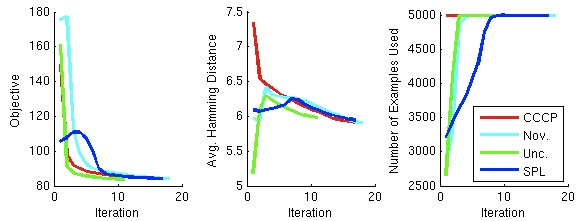
\includegraphics[scale = 0.7]{ExampleMotifRun_WithNovelty_small2.png}
\caption{Objective value, average Hamming distance, and number of included training examples in each outer iteration for the four learning algorithms on a single protein, fold, and seed.}
\label{fig:exrun}
\end{figure}

The rightmost plot shows that the addition of examples is much more gradual in slack-based SPL than in SPL-Uncertainty or SPL-Novelty, a result that holds across our runs. After just a couple of outer iterations, both the SPL-Uncertainty and SPL-Novelty algorithms had included all of the training examples. By examining the uncertainty, slack, and novelty values for the training examples over time, we identified the cause of this behavior: as better parameters are learned, the uncertainty and novelty drop much more quickly than the slack. Because SPL-Uncertainty adds all of the examples to the training set so quickly, the trajectory of its objective function during training looks more similar to that of CCCP than that of SPL. For instance, the ``hump'' in the objective curve characteristic of standard slack-based SPL is absent from the objective curve of the SPL-Uncertainty algorithm.

As another measure of performance, we considered the Hamming distance (the minimum number of substitutions required to convert one string to another of equal length) between motifs in positive examples. The middle plot in Figure \ref{fig:exrun} shows the average Hamming distance for selected samples over iterations. Consistent with the observations in \cite{SPL}, we saw that the Hamming distance for slack-based SPL tended to start low, increase as more difficult examples were introduced, and then decrease again once all examples had been included. For SPL-Uncertainty, due to the rapid introduction of all examples, we see only a brief increase in average Hamming distance followed by a longer period of decrease; in this respect, we again see that SPL-Uncertainty more closely resembles CCCP than it does slack-based SPL.  Note that the initially low Hamming distance for SPL-Uncertainty is a result of its preferential selection of negative sequences; these sequences do not have motifs and therefore are not included in the computation of Hamming distance.

\myparagraph{Rate of Inclusion.} One of our key observations from the analysis of single runs was that SPL-Uncertainty tends to add examples much more quickly than slack-based SPL. We hypothesized that the improved performance of SPL-Uncertainty relative to standard SPL could be caused by  \emph{faster inclusion} of all training examples, rather than by \emph{order of inclusion}.  To investigate this hypothesis, we ran slack-based SPL again with parameters that caused faster annealing: $\mu=2.0$ instead of $\mu=1.3$ in the original.  The results are shown in Table \ref{tbl:faster}.  With faster annealing, slack-based SPL performs better on two proteins, worse on two, and identically on one. SPL-Uncertainty outperforms both versions of slack-based SPL.  This result suggests that the better performance of SPL-Uncertainty was a function of the order of example inclusion, rather than rate of inclusion.

\myparagraph{Order of Inclusion.} Since annealing rate didn't appear to be the primary factor in why SPL-Uncertainty outperforms slack-based SPL, we sought to understand how these criteria differ in \emph{order of inclusion}. To answer this question, we plotted the order in which samples are first selected by one criterion against another, as shown in Figure~\ref{fig:order}. A point at ($i$, $j$) indicates that the $i$-th example selected by criteria {\sc X} was the $j$-th example selected by criteria {\sc Y}.  If the criteria are equal the plot is the line $y=x$, and if they are totally unrelated, the plot is white noise.  In SPL, examples are actually added in batches, so within a batch we ordered examples by increasing criterion value at time of addition.  Further, in SPL an example may be included one iteration, then rejected in a later iteration, then included again.  To let us draw meaningful comparisons between orderings for two different criteria, we included an example in the ordering exactly once corresponding to the first iteration in which it was included.  Finally, because there is only uncertainty over $\bf h$ in positive DNA sequences, we only compare the order of inclusion of those sequences.

\begin{figure}
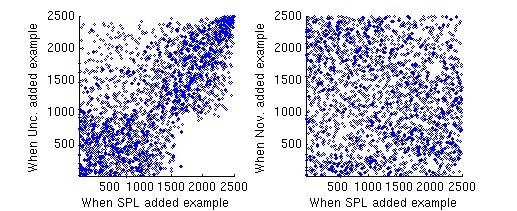
\includegraphics{ordercomp.png}
\caption{Comparison of order of inclusion of training examples for standard slack-based SPL and our two new selection criteria, uncertainty (Unc) and novelty (Nov).}
\label{fig:order}
\end{figure}

We first compared the best two selection criteria, slack and uncertainly, in the left plot of Figure~\ref{fig:order}.  We observe that they select from similar pools of points in the first and second halves of their training, as revealed by the two rectangular blocks in the bottom left and top right of the plot. Within these blocks, the points seem to be uniformly scattered. On the whole, the plot suggests that slack and uncertainty are at least somewhat similar, which helps us understand how both algorithms do significantly better than {\sc CCCP} at avoiding very bad local optima.  Interestingly, the two orderings agree most tightly on the very hardest samples, leading to a cluster in the top right of the graph.  This observation suggests that the gain of SPL may come more from excluding very hard samples for as long as possible rather than choosing very easy ones early on.

We also compared the order of selection for SPL-Novelty and slack-based SPL in the right plot of Figure~\ref{fig:order}. The plot suggests that novelty and slack are weakly inversely related: higher densities of points in the top left and bottom right quadrants indicate that examples chosen early by slack are more likely to be chosen late by novelty, and vice versa.  One possible explanation is that novelty selects examples with large $\|\Phi\|$, since the same $\Delta w$ will achieve a bigger $\Delta w^\top\Phi$ for such examples.  These examples are also likely to have large slack, so they will be chosen late by slack-based SPL.

\myparagraph{A Second Application: Bounding Boxes.} We observed that SPL-Uncertainty performed well for the motif finding problem and wanted to determine whether its strong performance would generalize to other problems. To answer this question, we applied SPL-Uncertainty to the object localization problem described in \cite{SPL}. In this problem, the examples are images containing objects of a particular type (in our experiment, each image contained a certain type of mammal), and the goal is to determine which type of object each image contains. The hidden variable is the location of the bounding box surrounding the object. Our dataset, as in \cite{SPL}, consisted of 271 images, each one containing one of 6 mammals. We used five folds (90\% train, 10\% test) to evaluate the algorithms and obtained the results displayed in Table \ref{tbl:bbox}. On average, the SPL-Uncertainty algorithm obtained higher final objective values than standard SPL. The two algorithms had the same average train and test set errors, and SPL-Uncertainty converged in much less time. Notably, the SPL-Uncertainty algorithm converged even faster than CCCP on average.

In this application, the use of entropy is confounded by the fact that bounding boxes very near to each other will achieve similar scores, possibly leading to a high uncertainty score even when we are confident about the general bounding box location. (This is not an issue in the motif finding application, in which neighboring subsequences will have very different feature vectors $\Phi$.)  We believe that addressing this problem with a non-maximum suppression technique could lead to improved performance of SPL-Uncertainty in this application. 

\mysection{Conclusion}
\label{sec:conclusion}

We have explored two novel inclusion criteria for Self-Paced Learning ({\sc SPL}): \textbf{uncertainty} and \textbf{novelty}. Novelty performed poorly relative to slack by getting stuck in bad local optima in over half of its runs, exactly the opposite of the goal of SPL. We believe that this is because the novelty criteria preferentially chooses training examples that don't change $\bf w$ much, essentially `trying to get stuck.' Novelty, therefore, does not seem to be a promising avenue for further research.

On the other hand, the uncertainty-based SPL performed very well. In the motif finding application, the uncertainty criterion generally led to improved objective value, lower train and test error, lower run time, and avoidance of getting stuck at very bad local optima. In the object localization problem, uncertainty-based SPL performed slightly worse than standard SPL in terms of objective value, but ran much more quickly and achieved the same train and test errors. Based on these results, the uncertainty criterion is a promising one that merits larger-scale investigation. Given the widespread applications of latent SSVM, improving the SPL algorithm with this new selection criterion has the potential to pay dividends in many areas. 

\myparagraph{Acknowledgements.}
Thanks to Pawan Kumar and Ben Packer for being generous with their code, time, and expertise.

\appendix

\newpage

\mysection{Algorithms}
\label{sec:algs}

\begin{algorithm}[h!]
\mytopcaption{Outer Loop: The self-paced learning algorithm for parameter estimation of latent {\sc ssvm}.}
\label{algo:selfPacedLatentSSVM}
\begin{algorithmic}[1]
\INPUT ${\cal D} = \{({\bf x}_1,{\bf y}_1),\cdots,({\bf x}_n,{\bf y}_n)\}$, ${\bf w}_0$, $K_0$, $\epsilon$, $\mu$.
\STATE $t \leftarrow 0$, $K \leftarrow K_0$.
\REPEAT
\STATE Update $h_i^* = \argmax_{h_i \in {\cal H}} {\bf w}_{t}^\top \Phi({\bf x}_i,{\bf y}_i,{\bf h}_i)$ for all $i$.
\STATE Update ${\bf w}_{t+1}$ by using {\sc acs} to minimize the objective
$\frac{1}{2}||{\bf w}||^2 + \frac{C}{n} \sum_{i=1}^n v_i\xi_i$ subject to the contraints in~(\ref{eq:latentSSVM}) and $v_i=I\left\{f({\bf x_i,\bf y_i;\bf w}) < \frac{1}{K}\right\}$.
\STATE $t \leftarrow t + 1$, $K \leftarrow K/\mu$.
\UNTIL{$v_i = 1, \forall i$ and the objective function cannot be decreased below tolerance $\epsilon$.}
\end{algorithmic}
\end{algorithm}


\begin{algorithm}[h!]
\mytopcaption{Inner Loop: Parameter estimation and example inclusion in \sc{SPL}.}
\label{algo:latentSSVM}
\begin{algorithmic}[1]
\INPUT ${\cal D} = \{({\bf x}_1,{\bf y}_1),\cdots,({\bf x}_n,{\bf y}_n)\}$, ${\bf w}_0$, $\epsilon$, $h_i^*$.
\STATE $t \leftarrow 0$
\REPEAT
\STATE Update $v_i = 1$ if $f({\bf x_i, \bf y_i;\bf w_t}) < \frac{1}{K}$, $v_i=0$ otherwise.  Recall that $f$ is the `difficulty' of a sample.
\STATE Update ${\bf w}_{t+1}$ by solving the corresponding
{\sc ssvm} problem over the samples with $v_i=1$. Specifically, \\
${\bf w}_{t+1} = \argmin_{\bf w} \frac{1}{2}||{\bf w}||^2 + \frac{C}{n}\sum_{i} v_i\max\{0,\Delta({\bf y}_i,\hat{\bf y}_i) +
		{\bf w}^\top (\Phi({\bf x}_i,\hat{\bf y}_i,\hat{\bf h}_i) - \Phi({\bf x}_i,{\bf y}_i,{\bf h}_i^*))\}$.
\STATE $t \leftarrow t + 1$.
\UNTIL{Objective function cannot be decreased below tolerance $\epsilon$.}
\end{algorithmic}
\end{algorithm}


\newpage

\mysection{Tables}
\label{sec:tables}



\begin{table}[h]
\begin{center}
\subfigure[Final Objective Values] {
\begin{tabular}{|c|c|c|c|c|c|}
\hline Protein Number  & CCCP & SPL & Uncertainty & Novelty \\\hline
1 & \textbf{57.49} $\pm$ \textbf{1.70} & $57.78 \pm 1.48$ & $57.52 \pm 1.67$ & $95.01 \pm 45.06$\\
2 & $85.04 \pm 2.73$ & $84.67 \pm 3.14$ & \textbf{83.89} $\pm$ \textbf{2.26} & $84.08 \pm 1.14$\\
3 & $91.32 \pm 29.58$ & $78.27 \pm 4.51$ & \textbf{75.33} $\pm$ \textbf{4.27} & $105.63 \pm 36.40$\\
4 & $94.63 \pm 27.74$ & $79.93 \pm 1.59$ & \textbf{79.27} $\pm$ \textbf{1.06} & $80.45 \pm 2.81$\\
5 & $73.86 \pm 38.07$ & $54.26 \pm 1.09$ & \textbf{54.04} $\pm$ \textbf{0.84} & $111.90 \pm 46.77$ \\\hline
\end{tabular}
}
\subfigure[Train Errors (\%)] {
\begin{tabular}{|c|c|c|c|c|c|}
\hline Protein Number  & CCCP & SPL & Uncertainty & Novelty \\\hline
1 & $12.74 \pm 0.79$ & $12.79 \pm 0.75$ & \textbf{12.66} $\pm$ \textbf{0.74} & $27.76 \pm 18.17$\\
2 & $23.68 \pm 1.32$ & $23.07 \pm 1.27$ & \textbf{22.62} $\pm$ \textbf{0.90} & $23.01 \pm 0.33$\\
3 & $25.58 \pm 12.28$ & $19.90 \pm 1.76$ & \textbf{19.07} $\pm$ \textbf{1.65} & $31.49 \pm 15.14$\\
4 & $26.38 \pm 11.22$ & $21.30 \pm 1.57$ & ${20.46} \pm {0.58}$ & \textbf{20.33} $\pm$ \textbf{0.52}\\
5 & $20.27 \pm 14.88$ & $12.56 \pm 0.46$ & \textbf{12.49} $\pm$ \textbf{0.15} & $35.14 \pm 18.20$\\\hline
\end{tabular}
}
\subfigure[Test Errors (\%)] {
\begin{tabular}{|c|c|c|c|c|c|}
\hline Protein Number  & CCCP & SPL & Uncertainty & Novelty \\\hline
1 & \textbf{31.65} $\pm$ \textbf{0.43} & $31.77 \pm 0.47$ & \textbf{31.65}$\pm$ \textbf{0.35} & $39.03 \pm 8.96$\\
2 & $31.44 \pm 0.40$ & \textbf{30.83} $\pm$ \textbf{0.27} & $31.02 \pm 0.18$ & $31.44 \pm 0.36$\\
3 & $33.79 \pm 8.12$ & $30.33 \pm 0.77$ & \textbf{29.85} $\pm$ \textbf{0.51} & $37.99 \pm 9.82$\\
4 & $34.95 \pm 7.12$ & $31.49 \pm 0.30$ & \textbf{31.43} $\pm$ \textbf{0.43} & $31.38 \pm 0.58$\\
5 & $32.36 \pm 8.83$ & $27.97 \pm 0.27$ & \textbf{27.90} $\pm$ \textbf{0.28} & $41.22 \pm 10.76$\\\hline
\end{tabular}
}
\subfigure[Run Times (seconds)] {
\begin{tabular}{|c|c|c|c|c|c|}\hline
 CCCP & SPL & Uncertainty & Novelty \\\hline
$\bf 397.35 \pm 291.37$ & $642.61 \pm 330.48$ & $460.10 \pm 237.29$ & $3085.39 \pm 3151.12$\\\hline
\end{tabular}
}
\end{center}
\caption{The results (reported as mean $\pm$ standard deviation) for the four algorithms in the motif finding application. In general, the SPL-Uncertainty algorithm outperformed the other three and ran faster than the original SPL algorithm.  The best result in each row appears in \textbf{bold}. }
\label{tbl:motif}
\end{table}



\begin{table}[h]
\caption{The results (reported as mean $\pm$ standard deviation) of slack-based SPL with a normal and high annealing rate $\mu$. The corresponding SPL-Uncertainty results are included for reference (shown in \emph{italics} to avoid confusion). The performance of SPL was similar for both annealing rates, with the better slack result in \textbf{bold}.  SPL-Uncertainty outperforms slack-based SPL on 4 of 5 proteins.}
\begin{center}
\begin{tabular}{|c|c|c|c|c|c|}
\hline Protein Number  & SPL ($\mu=1.3$) & SPL ($\mu=2.0$) & Uncertainty ($\mu=1.3$) \\\hline
1 & ${\bf57.78 \pm 1.48}$ & $57.84 \pm 1.50$ & $\it{57.52 \pm 1.67}$ \\ \hline
2 & ${\bf84.67 \pm 3.14}$ & $84.83 \pm 3.30$ & $\it{83.89 \pm 2.26}$ \\ \hline
3 & $78.27 \pm 4.51$ & ${\bf76.42 \pm 4.24}$ & $\it{75.33 \pm 4.27}$ \\ \hline
4 & ${\bf79.93 \pm 1.59}$ & ${\bf79.93 \pm 1.57}$ & $\it{79.27 \pm 1.06}$ \\ \hline
5 & $54.26 \pm 1.09$ & ${\bf54.02 \pm 1.12}$ & $\it{54.04 \pm 0.84}$ \\ \hline
\end{tabular}
\end{center}
\label{tbl:faster}
\end{table}


\begin{table}[h]
\caption{The results (reported as mean $\pm$ standard deviation) for the three algorithms in the object localization problem. The standard SPL algorithm outperformed SPL-Uncertainty in terms of final objective value, but the SPL-Uncertainty algorithm ran significantly faster and obtained equivalent train and test errors.}
\begin{center}
\begin{tabular}{|c|c|c|c|}
\hline  & CCCP & SPL & Uncertainty \\\hline
Final Objective & $4.70 \pm 0.10$ & \textbf{4.42} $\pm$ \textbf{0.11} & $4.47 \pm 0.08$ \\\hline
Train Error (\%) & $0.33 \pm 0.16$ & \textbf{0.08} $\pm$ \textbf{0.16} & \textbf{0.08} $\pm$ \textbf{0.16}  \\ \hline
Test Error (\%) & $16.92 \pm 4.62$ & \textbf{16.15} $\pm$ \textbf{6.15} & \textbf{16.15} $\pm$ \textbf{6.16} \\ \hline
Run Time (sec) & $858.96 \pm 140.62$ & $1421.66 \pm 100.14$ & \textbf{544.32} $\pm$ \textbf{36.27} \\ \hline
\end{tabular}
\end{center}
\label{tbl:bbox}
\end{table}



\newpage
 
\begin{thebibliography}{9}


\bibitem{SPL} P Kumar, B Packer, and D Koller. \emph{Self-Paced Learning for Latent Variable Models},
NIPS 2010. \url{http://ai.stanford.edu/~koller/Papers/Kumar+al:NIPS10.pdf}

\bibitem{SSVM} CN Yu, T Joachims. \emph{Learning Structural SVMs with Latent Variables}. \url{www.cs.cornell.edu/~cnyu/papers/icml09_latentssvm.pdf}

\bibitem{App1} PF Felzenszwalb, RB Girshick, D McAllester and D Ramanan. \emph{Object Detection with Discriminatively Trained
Part Based Models}.  \url{http://www.ics.uci.edu/~dramanan/papers/latentmix.pdf}

\bibitem{Mosek} The MOSEK Optimization Software. \url{http://www.mosek.com/}

\end{thebibliography}

\end{document}